\chapter{Quantum Error Correction with GKP Codes\label{ch:2_QEC}}

\section{General Notions of QEC}
It is sometimes said that the concept of quantum error correction is more remarkable than the concept of quantum computation itself \cite{girvin2019QECvideo}. Indeed, the fact that quantum error correction is in principle even possible is somewhat surprising, for three fundamental reasons: (1) the \textit{no-cloning} theorem \cite{ike-and-mike}, which forbids us from copying unknown quantum states to naively add redundancy; (2) the \textit{measurement problem}, also known as Born's rule, whereby measuring a quantum state causes it to collapse due to measurement backaction; and (3) errors on quantum states can be continuous-valued and are thus in some sense analog. Despite these somewhat severe restrictions imposed by quantum mechanics, quantum error correction (QEC) can still be realized --- and, in fact, has been done so.


In this thesis, we are concerned with a specific class of quantum error correcting codes called \textit{bosonic codes}, which store information in the continuous-variable degree of freedom of a quantum harmonic oscillator. Specifically, among the various bosonic codes that exist, we will focus on the so-called Gottesman-Kitaev-Preskill (GKP) grid code and its practical realization in experiment. In this chapter, we will introduce the basic notions of bosonic QEC and the GKP code, study specific theoretical proposals for error correction of the GKP codewords, and discuss various challenges and experimental considerations.


\subsection{Qubits and the Errors that Befall Them}

\todo{Refer to QIS textbook to write this section.} Plan: Introduce qubit operators like $\sigma_z$ etc. since we'll use them throughout. Talk about quantum gates, quantum channels, Krauss maps, amplitude damping, dephasing, $T_1$, and $T_2$ for a 2-level qubit. 


\subsection{The Knill-Laflamme Condition for QEC}

\todo{Decide whether or not to skip this section}


\section{Overview of Bosonic Error Correction}
\subsection{Definitions and Notation \label{sec:2_BosonicQEC_Definitions}}
Here, we collect various definitions and identities from quantum optics that will be relevant to the discussion of bosonic QEC. Additional details can be found in Refs. \cite{shankar1994principles, raimond2006exploring, grynberg2010introduction}. We begin with an overview of the quantum harmonic oscillator, which is defined in terms of generalized position $\hat{x}$ and momentum $\hat{p}$ operators satisfying the commutation relation $[\hat{x}, \hat{p}] \equiv \hat{x}\hat{p} - \hat{p}\hat{x} = i\h$. The quantum Hamiltonian is given by
\begin{equation}
    \hat{H} = \frac{\hat{p}^2}{2m} + \frac{1}{2}m\omega^2 \hat{x}^2
\end{equation}
where $m$ denotes the mass and $\omega$ is the natural frequency \cite{shankar1994principles}. This is fully analogous to the classical Hamiltonian of a harmonic oscillator that we might study in a course on classical mechanics. In the quantum case, however, the oscillator will have quantized energy levels, which can be seen by introducing mode operators $\hat{a}, \hat{a}^\dagger$ that diagonalize the Hamiltonian:
\begin{align}
\begin{split}
     \hat{x} &= \sqrt{\frac{\h}{2m\omega}}(\hat{a} + \hat{a}^\dagger) \,\triangleq\, x_{\rm zpf} (\hat{a} + \hat{a}^\dagger) \\
     \hat{p} &= i\sqrt{\frac{m\h\omega}{2}}(\hat{a}^\dagger - \hat{a}) \,\triangleq\, \frac{i}{2x_{\rm zpf}} (\hat{a}^\dagger - \hat{a})
\end{split}
\end{align}
The commutation relation between $\hat{x}$ and $\hat{p}$ translates into an important relation: $[\hat{a}, \hat{a}^\dagger] = 1$. In quantum optics, it is also common convention to set $m, \omega, \h \to 1$, such that $x_{\rm zpf} \to 1/\sqrt{2}$. With these definitions in place, the oscillator Hamiltonian above takes on a simple form:
\begin{equation}
    \hat{H} = \h\omega\bigg(\hat{a}^\dagger\hat{a} + \frac{1}{2}\bigg) \,\triangleq\, \h\omega\bigg(\hat{n} + \frac{1}{2}\bigg)
\end{equation}
Here, we have defined the photon number operator $\hat{n} = \hat{a}^\dagger\hat{a}$ which tells us how many excitation quanta occupy an oscillator state. The energy eigenstates $\ket{n}$ (also known as \textit{Fock} states) satisfy $\hat{n}\ket{n} = n\ket{n}$, and thus the oscillator Hamiltonian satisfies $\hat{H}\ket{n} = E_n\ket{n}$ with energy levels $E_n = \h\omega(n + 1/2)$. The constant term $\h\omega/2$ is known as the zero-point energy; we mostly ignore it so that the oscillator Hamiltonian simplifies to just $\hat{H} = \h\omega \hat{a}^\dagger\hat{a}$. The mode operators $\hat{a}^\dagger, \hat{a}$ are referred to as \textit{creation} and \textit{anniliation} operators, since they act on Fock states via
\begin{equation}
    \hat{a}^\dagger\ket{n} = \sqrt{n+1}\ket{n+1}, \quad \hat{a}\ket{n} = \sqrt{n}\ket{n}.
\end{equation}
The Fock states $\{\ket{n}\}_{n=0}^\infty$ can be shown to form a basis for the formally infinite-dimensional Hilbert space $\mathcal{H}$ of a single oscillator mode; thus, $\ip{m}{n} = \delta_{n, m}$ and $\sum_n \op{n}{n} = \hat{I}$, where $\delta_{n, m}$ is the Kronecker delta and $\hat{I}$ is the identity operator on $\mathcal{H}$. 

In analogy with a classical oscillator, we can also define the \textit{position} and \textit{momentum} states of the quantum harmonic oscillator via the set of non-normalizable eigenstates $\ket{x}$ and $\ket{p}$, which satisfy $\hat{x}\ket{x} = x\ket{x}$ and $\hat{p}\ket{p} = p\ket{p}$ for $x, p \in \R$. These continuous-variable oscillator states satisfy
\begin{equation}
    \int_{x \in \R} \op{x}{x}dx = \int_{p \in \R} \op{p}{p} dp = \hat{I}
\end{equation}
and, like any conjugate pair of variables in quantum mechanics, can be related via Fourier transform: $\ket{x} = \frac{1}{\sqrt{2\pi}} \int_p dp e^{-ipq}\ket{p}$. One important set of identities the eigenstates $\ket{x}$ and $\ket{p}$ is the following: 
\begin{equation}
    e^{-iu\hat{p}}\ket{x} = \ket{x + u}, \quad e^{iv\hat{x}}\ket{p} = \ket{p+v}
\end{equation}
Effectively, the operators $\exp(-iu\hat{p})$ and $\exp(iv\hat{x})$ enable us to shift the position and momentum of the oscillator by $u$ and $v$ respectively. We can combine both into a quadrature displacement operator $\hat{D}(u, v) \equiv \exp(iv\hat{x} - iu\hat{p})$. Setting $\alpha = (u+iv)/\sqrt{2}$, we can then define the phase-space displacement operator $\hat{D}(\alpha) \equiv \hat{D}(u, v)$ as follows: 
\begin{equation}
    \hat{D}(\alpha) = \exp(\hat{a}^\dagger \alpha - \alpha^\ast \hat{a})
\end{equation}
Written in this canonical form, the displacement operator has several useful identities. In particular,  we have $\hat{D}^\dagger(\alpha) = \hat{D}(-\alpha)$ and $\hat{D}^\dagger(\alpha) \hat{a} \hat{D}(\alpha) = \hat{a} + \alpha$. The displacement operator also generates so-called \textit{coherent states} $\ket{\alpha} \equiv \hat{D}(\alpha)\ket{0}$ when operated on the vacuum state $\ket{0}$. These coherent states are eigenstates of $\hat{a}$, satisfying $\hat{a}\ket{\alpha} = \alpha\ket{\alpha}$, and can be explicitly constructed via:
\begin{equation}
    \ket{\alpha} = e^{-|\alpha|^2/2}\sum_{n=0}^\infty \frac{\alpha^n}{\sqrt{n!}} \ket{n}
\end{equation}

\noindent \textbf{Visualizing oscillator states.} In this section, we have introduced Fock states and coherent states as two important classes of oscillator states. For more general mixed states, we also typically represent oscillator states using a density matrix $\rho$. However, by far the most intuitive way to describe and visualize bosonic states is to use a phase-space quasiprobability distribution. One of the most common is the symmetric characteristic function $C(\beta)$, defined via: 
\begin{equation}
    C(\beta) = \ev{\hat{D}(\beta)} = \Tr[\rho \hat{D}(\beta)] 
\end{equation}
By taking the two-dimensional Fourier transform of this function in phase space, we arrive at the Wigner function
\begin{equation}
    W(\alpha) = \frac{1}{\pi^2}\int C(\beta) e^{\alpha\beta^\ast - \alpha^\ast\beta} d^2\beta
\end{equation}
By plotting $W(\alpha)$ as a function of $x = \sqrt{2}\mathrm{Re}(\alpha)$ and $p = \sqrt{2}\mathrm{Im}(\alpha)$, we can visualize an oscillator state $\rho$ in phase space. The Wigner function has some nice mathematical properties \todo{list the properties; also mention marginal distributions; }

We also have \cite{royer1977wigner}:
\begin{equation}
    W(\alpha) = \frac{2}{\pi}\Tr\big[\hat{D}(-\alpha)\hat{\rho}\hat{D}(\alpha)\hat{\Pi}]
\end{equation}
where $\hat{\Pi} = (-1)^{\hat{a}^\dagger\hat{a}}$ is the so-called parity operator. This is easy to measure in circuit QED \cite{sun2014tracking}. 

\begin{figure}
    \centering
    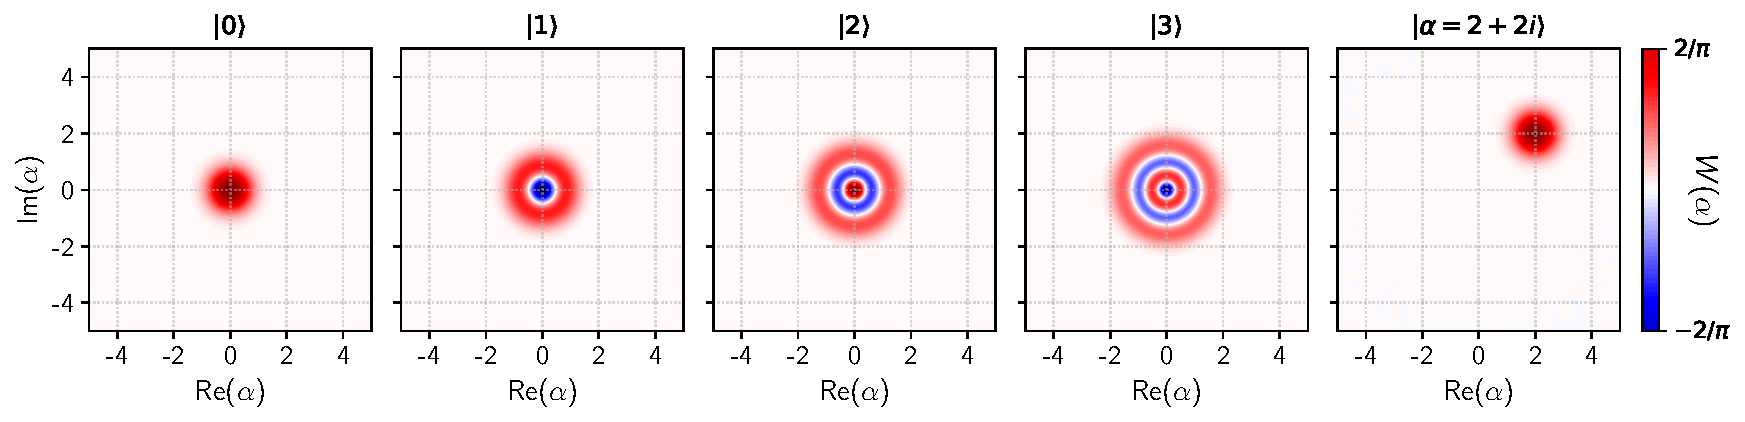
\includegraphics[width=\linewidth]{Figures/2/Fock_Wigners.pdf}
    \caption{Caption}
    \label{fig:2_Fock_Wigners}
\end{figure}

\subsection{Control, Nonlinearity, and Auxiliary Qubits\label{sec:2_control_nonlinearity_drive}}
In circuit QED, we usually control harmonic oscillators by subjecting them to a microwave drive on one of its quadratures \cite{manenti2023quantum}. Specifically, we end up implementing a Hamiltonian of the form:
\begin{equation}
    \hat{H}(t) = \hat{H}_{\rm QHO} + \hat{H}_d(t) = \omega_a \hat{a}^\dagger \hat{a} + \epsilon(t)(\hat{a} + \hat{a}^\dagger)\cos(\omega t)
    \label{eq:2_oscillator_drive}
\end{equation}
consisting of a bare quantum harmonic oscillator (note that we have set $\h \to 1$, to equate energies and frequencies here), as well as a drive Hamiltonian $\hat{H}_d(t)$ that modulates one of the quadratures, i.e. $\hat{x} \sim \hat{a} + \hat{a}^\dagger$ in this case\footnote{Later in our chapter on circuit QED, it will be more typical to couple to the $\hat{p} \sim i(\hat{a}^\dagger - \hat{a})$, which corresponds to the ``charge'' of the electrical implementation of the quantum harmonic oscillator, known as an LC circuit.}. Typically, this is only form of control that we can implement over a linear oscillator, and as we will now see, results in a displacement of the oscillator in phase space. In order to drive excitations of the system, we ideally want a resonant drive (as we did for the qubit), i.e. so that $\omega = \omega_a$. In this case, we can transform to the so-called \textbf{rotating frame} via the unitary operator $\hat{U}(t) = \exp[-i\omega t\hat{a}^\dagger \hat{a}]$ to analyze the dynamics. Since we have not yet encountered this concept in this thesis, let's now discuss it. Essentially, we can think of $\hat{U}(t)$ as a change of basis, i.e. a canonical transformation to a moving frame of reference where the quadrature axes of phase space are now themselves also rotating at frequency $\omega$. In our case, working in the ``Heisenberg picture'' of quantum mechanics at the level of operators, the effect of the time-dependent unitary $\hat{U}(t)$ is to map the Hamiltonian
\begin{equation}
    \hat{H} \mapsto \hat{U} \hat{H} \hat{U}^\dagger + i[\partial_t \hat{U}]\hat{U}^\dagger
\end{equation}
where the first term captures the change of basis and the second term is a time-dependent correction in this frame; it is analogous to, for example, a Coriolis force that arises when moving to a non-inertial frame of reference in classical mechanics \cite{goldstein-classical-mechanics}. 

Returning now to our treatment of drives in an oscillator, we can now analyze the driven QHO via:
\begin{equation}
    \hat{H}(t) \mapsto \hat{H}_{\rm rot}(t) = (\omega_a - \omega)\hat{a}^\dagger \hat{a} + \epsilon(t)(\hat{a} e^{-i\omega t} + \hat{a}^\dagger e^{i\omega t})\cos(\omega t)
\end{equation}
in the rotating frame, where $\hat{U}(t)$ has the effect of transforming $\hat{a} \mapsto a e^{-i\omega t}$. When $\omega = \omega_a$, the frame-dependent correction term exactly cancels with the bare oscillator Hamiltonian $\hat{H}_{\rm QHO}$. Meanwhile, by expanding $\cos(\omega t) = (e^{i\omega t} + e^{-i\omega t})/2$, we see that the resulting drive term will have a static component and components rotating with frequencies $e^{\pm 2i\omega t}$. In the resonant case we are in, these terms will be fast-oscillating and highly off resonant; we can thus often neglect them, making the famous rotating-wave approximation (RWA)\footnote{The RWA works very well in many cases, but also has its limits where the so-called counter-rotating terms at frequencies $\pm 2\omega$ cannot be ignored. We will return to the RWA many more times throughout this thesis.}. If we do this here, we are left with
\begin{equation}
    \hat{H}_{\rm rot} = \frac{\epsilon(t)}{2} \big(\hat{a} + \hat{a}^\dagger\big)
\end{equation}
where the only remaining time-dependence is the slow variation of the drive \textit{envelope} $\epsilon(t)$. If we now solve the Schr\"odinger equation $i\partial_t \ket{\psi} = \hat{H}_{\rm rot}\ket{\psi}$ with this Hamiltonian using a constant drive $\epsilon(t) = \epsilon_0$, we get the expected unitary evolution $\ket{\psi(t)} = \hat{U}_{\rm p}(t) \ket{\psi(0)}$ with the propagator given by $\hat{U}_{\rm p}(t) = \exp[-i\hat{H}_{\rm rot} t]$. We can confirm that this has the form of an oscillator displacement
\begin{equation}
    \hat{U}_{\rm p}(t) = e^{-i\epsilon_0 t(\hat{a} + \hat{a}^\dagger)/2} = \hat{D}\bigg(\frac{-i\epsilon_0 t}{2}\bigg)
\end{equation}
from which we conclude that any initial oscillator state will simply just be displaced under the action of a resonant drive. In particular, starting from the vacuum state $\ket{0}$, we have no way to prepare the Fock $\ket{1}$ state, since all higher energy levels of a linear oscillator by definition have the same frequency spacing $\omega_a$ as the $\ket{0}\to\ket{1}$ transition. Given this, it is not immediately clear how we can realize universal control and prepare nontrivial states of the oscillator for the purpose of bosonic quantum error correction.

It turns out the solution to this is to \textit{introduce} some form of nonlinearity into the oscillator, typically by coupling it to some auxiliary nonlinear element such as a two-level qubit/spin \cite{cai2021bosonic, raimond2006exploring, haroche2020cavity, blais2021circuit}. This approach was pioneered in Cavity QED experiments in the 1990s and later adopted by circuit QED. We can get an intuitive understanding by considering the basic foundational model for coupling an oscillator to a qubit, known as the Jaynes-Cummings Hamiltonian \cite{raimond2006exploring}:
\begin{equation}
    \hat{H}_{\rm JC} = \omega_a \hat{a}^\dagger\hat{a} + \frac{\omega_q}{2}\sigmaz + g(\hat{a}^\dagger\sigmam + \hat{a}\sigmap)
\end{equation}
Here, the interaction is mediated via an operator that swaps excitations between the qubit and the oscillator. In circuit QED, we usually work in the off-resonant regime $g \ll |\omega_a - \omega_q|$; but if we briefly imagine somehow bringing the qubit into resonance with the oscillator, we are left with $g(\hat{a}^\dagger\sigmam + \hat{a}\sigmap)$ in the interaction frame. Loosely speaking, we can populate the qubit (which, due to its inherent nonlinearity, may be done using just a resonant drive), and then swap the excitation to the oscillator via the exchange interaction. If we repeat this many times, we can imagine ``climbing the ladder'' of Fock levels to to prepare nontrivial states of the joint qubit-oscillator system \cite{krause1989preparation, meystre1990cat, vogel1993quantum}. In fact, this was one of the first methods for realizing universal control over an oscillator \cite{law1996arbitrary}. 

Of course, this intuitive explanation relies on the resonant Jaynes-Cummings interaction and thus does not work in the more typical \textit{dispersive regime} where the oscillator and qubit are far-detuned, i.e. $g \ll |\omega_a - \omega_q|$. In this case, however, it is possible to approximate the Jaynes-Cummings Hamiltonian by treating the interaction as a perturbation and going to second-order in perturbation theory \cite{raimond2006exploring}. Doing this leaves with us the effective dispersive Hamiltonian
\begin{equation}
    \hat{H}_{\rm disp} = \omega_a \hat{a}^\dagger\hat{a} + \frac{\omega_q}{2}\sigmaz + \frac{\chi}{2}\hat{a}^\dagger\hat{a}\sigmaz
    \label{eq:2_dispersive_model_qubit}
\end{equation}
where the so-called \textit{dispersive shift} $\chi$ is defined here as $\chi = 2g^2/(\omega_q - \omega_a)$. There is a lot to be said about Eq. \eqref{eq:2_dispersive_model_qubit}, as it is arguably the foundation on which almost all of modern circuit QED is built \cite{blais2004cavity}. The basic idea is that the effective oscillator frequency $\omega_a + \chi\sigmaz/2$ now depends on the qubit state via $\ev{\sigmaz}$, and in particular results in two different frequencies $\omega_a \pm \chi/2$ for when the qubit is in state $\ket{g}$ or $\ket{e}$ respectively. Equivalently, by regrouping the terms in Eq. \eqref{eq:2_dispersive_model_qubit} another way, the effective qubit frequency $(\omega_q + \chi \hat{a}^\dagger\hat{a})/2$ depends on the average number of photons $\ev{\hat{a}^\dagger\hat{a}}$ in the oscillator. The former grouping gives us a blueprint for the so-called \textit{dispersive readout} of a qubit, through which one may determine the qubit state just by measuring the frequency of a resonator that it is coupled to. We will return to this idea again later in this thesis, such as when we discuss circuit QED in Ch. \ref{ch:3_cQED} and when we present our experimentals in Ch. \ref{ch:4_3DGKP}. 

Finally, returning to the question of oscillator state preparation for bosonic QEC, it turns out that it is possible to achieve universal control over the joint qubit and oscillator Hilbert space just by using the dispersive interaction together with arbitrary single-qubit rotations and oscillator displacements \cite{vlastakis2015controlling, reinhold2019controlling, eickbusch2022fast}. We will discuss the specific control requirements for QEC with the GKP code in the coming sections. 

\subsection{Oscillator Error Mechanisms}

\todo{Introduce the master equation}


\section{A Brief Introduction to GKP Grid Codes\label{sec:2_Intro_to_GKP}}

The Gottesman-Kitaev-Preskill (GKP) grid code is a bosonic encoding that embeds a logical qubit nonlocally within the phase space of a harmonic oscillator. While the code itself has been known for two decades since the original proposal by Gottesman, Kitaev, and Preskill \cite{gottesman2001gkp} in 2001, it was only recently realized experimentally in trapped ions \cite{fluhmann2019gkp-expt, deneeve2022gkp-expt} and superconducting circuits \cite{campagne2020gkp-expt, sivak2023gkp-expt, nordquantique2023gkp-expt}. In this section, we will introduce the basic theory of the GKP code as well as its finite-energy counterpart, and then discuss the various components required for their experimental realization. 

\subsection{Ideal GKP Codes}
In general, GKP codes are defined by a lattice in the $(2N)$-dimensional phase space of $N$ quantum harmonic oscillators \cite{gottesman2001gkp, royer2022multimodegkp}. In this thesis, however, we will focus on the simplest case of a single oscillator ($N=1$) whose phase space is described by the quadrature coordinates $\hat{x}$ and $\hat{p}$ as discussed in Sec. \ref{sec:2_BosonicQEC_Definitions}. Following the original proposal of Gottesman, Kitaev, and Preskill, we can consider the square lattice with lattice constant $\ells = 2\sqrt{\pi}$ formed by the quadratures $\hat{x}$ and $\hat{p}$. The ideal GKP codewords associated with this lattice are defined as the simultaneous $+1$ eigenstates of the following two stabilizer operators: 
\begin{equation}
    \hat{S}_0^X = e^{-i\ells\hat{p}} = \hat{D}(\ell) , \qquad \hat{S}_0^Z = e^{i\ells\hat{x}} = \hat{D}(i\ell)
\end{equation}
where we define the reduced lattice constant $\ell = \ells/\sqrt{2}$ as the \textit{phase space} displacement associated with the quadrature displacement $\ell_s$. We can therefore write down the canonical GKP codewords directly. They are given by the $\hat{x}$ basis states
\begin{equation}
    \ket{0_L} \propto \sum_{j \in \Z} \ket{x = j\ells}, \qquad \ket{1_L} \propto \sum_{j \in \Z} \ket{x = (j + 1/2)\ells}.
    \label{eq:GKP_codewords_ideal}
\end{equation}
Together, these two codewords form a two-dimensional logical subspace $\mathcal{C} \equiv \{\ket{0_L}, \ket{1_L}\}$ within the infinite-dimensional Hilbert space $\mathcal{H}$ of the oscillator. We plot the wavefunctions for the codewords of Eq. \eqref{eq:GKP_codewords_ideal} in the position basis in Fig. \todo{make figure}, as well as the associated Wigner functions for the six cardinal states of the logical Bloch sphere: $\ket{\pm X_L}$, $\ket{\pm Y_L}$, and $\ket{\pm Z_L} \equiv \ket{0_L/1_L}$. By construction, we have $\hat{S}_0^X\ket{\mu_L} = \hat{S}_0^Z\ket{\mu_L} = \ket{\mu_L}$ for $\mu\in\{0, 1\}$, thus confirming that the operators $\hat{S}_0^X, \hat{S}_0^Z$ are indeed stabilizers. From Fig. \todo{make figure}, it is also clear that logical Pauli operators can be implemented via displacements of half the lattice constant: 
\begin{equation}
    \hat{X}_L^0 = \sqrt{\hat{S}_0^X} =  e^{-i\ells\hat{p}/2} , \qquad \hat{Z}_L^0 = \sqrt{\hat{S}_0^Z} = e^{i\ells\hat{x}/2}. 
\end{equation}

At this point, we might ask how the GKP states introduced above can be used for QEC. As originally proposed, the GKP code was designed to correct error channels that manifest as small phase space displacements of the oscillator, i.e. sending $(x, p) \to (x + \delta_x, p+\delta_p)$. The basic principle is as follows: observe that $[\hat{S}_0^Z, \hat{S}_0^X] = [e^{i\ells\hat{x}}, e^{-i\ells\hat{p}}] = 0$, i.e. the two GKP stabilizers commute and we can measure them simultaneously in their joint eigenbasis. This in turn implies that it is possible to measure $\hat{x}$ and $\hat{p}$ simultaneously as long as both are taken modulo $\ell/2$\footnote{Following \cite{royer2020gkp}, we will sometimes refer to the modular quadratures $\hat{x}_{[m]} \equiv \hat{x} \Mod m$ and $\hat{p}_{[m]} \equiv \hat{p} \Mod m$ with a symmetric modulo, i.e. $\hat{x}_{[m]}, \hat{p}_{[m]} \in [-m/2, m/2)$. We are specifically interested in $\hat{x}_{[\ells/2]}$ and $\hat{p}_{[\ells/2]}$.}. Therefore, if an error shifts the GKP grid $(x, p) \to (x + \delta_x, p+\delta_p)$, we can simply measure the modular quadratures and then apply a correction operation $\hat{D}(-\alpha)$ with $\alpha = (\delta_x + i\delta_p)/\sqrt{2}$ to re-center the grid. If the errors are small, i.e. $|\delta_x|, |\delta_p| < \ells / 4$, this results in a perfect recovery of the logical information, as depicted in Fig. \ref{fig:2-GKP-Ideal-QEC}(a). For realistic oscillators, most physical decoherence processes such as amplitude damping or dephasing occur via a continuous distortion of phase space, and can thus be corrected for if the GKP stabilizers are measured frequently enough \cite{gottesman2001gkp, glancy2006gkperror, albert2018performance-and-structure, noh2018performance-and-structure-pt2}. Among the various single-mode bosonic codes, it has been shown that the GKP code offers the best protection against photon loss, which is the dominant error mechanism for superconducting resonators \cite{albert2018performance-and-structure}. 
\begin{figure}[h]
    \centering
    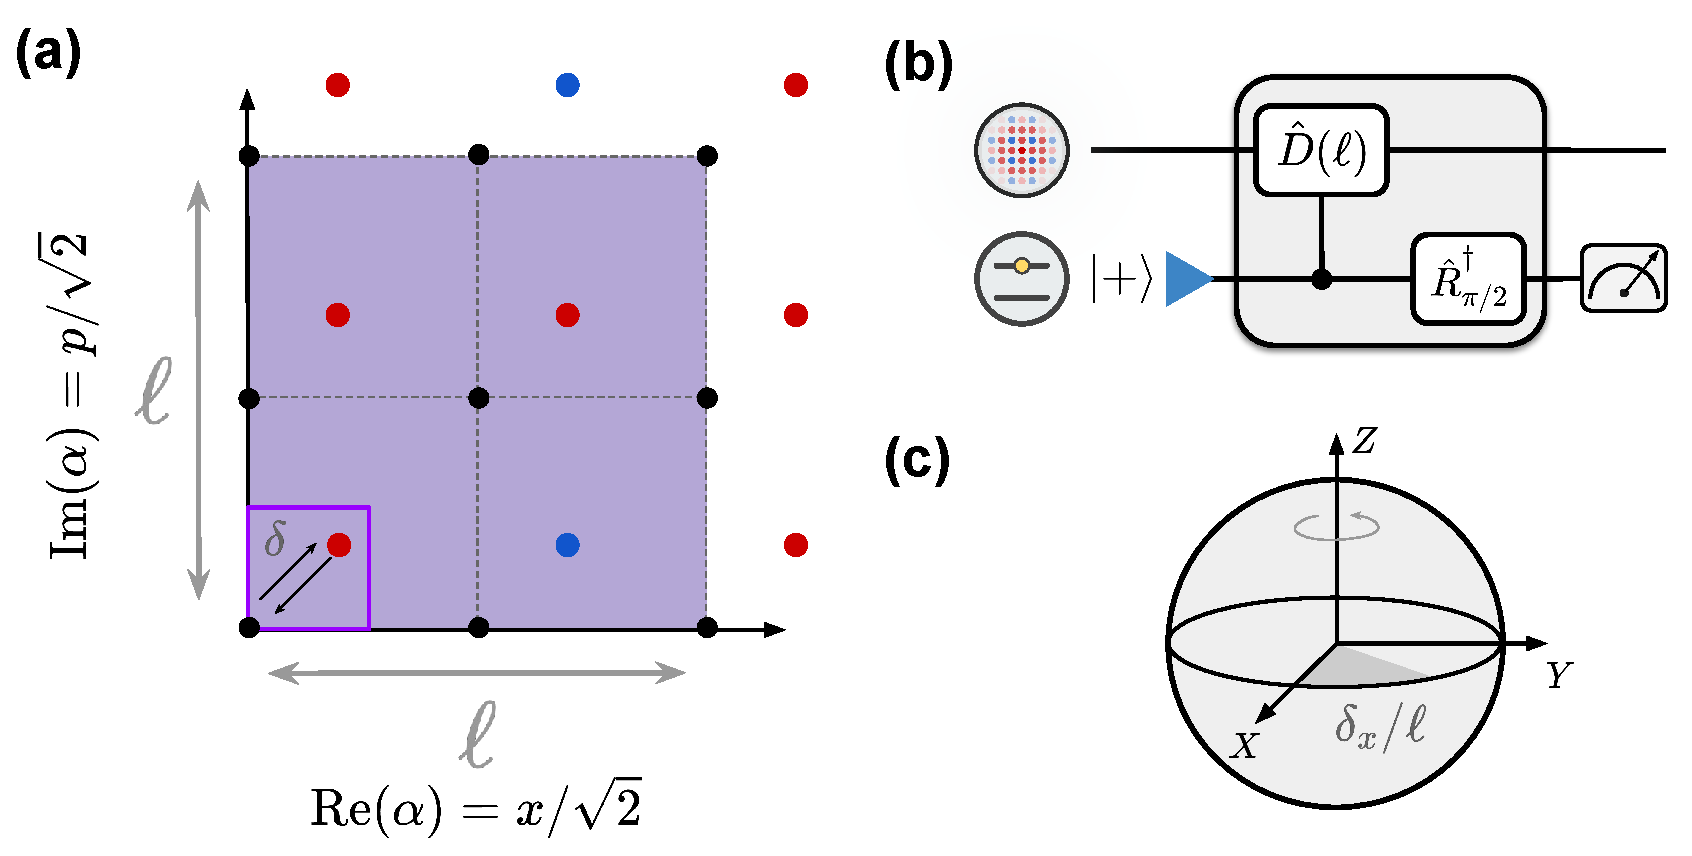
\includegraphics[width=\linewidth]{Figures/2/GKP Ideal QEC.pdf}
    \caption{\todo{caption}}
    \label{fig:2-GKP-Ideal-QEC}
\end{figure}

For an ideal GKP code, the actual stabilizer measurements can be carried out by using an auxiliary qubit as shown in Fig. \ref{fig:2-GKP-Ideal-QEC}(b). This circuit uses maps the stabilizer information onto the phase of the qubit using a conditional displacement operation
\begin{equation}
    {\rm CD}(\ell) = \hat{D}\bigg(\frac{\ell}{2}\bigg)\op{g}{g} + \hat{D}\bigg(\frac{-\ell}{2}\bigg)\op{e}{e} = \exp[\ell(\hat{a}^\dagger - \hat{a}) \sigmaz / 2].
    \label{eq:2_CD_unitary_definition}
\end{equation}
From the perspective of the oscillator, the CD gate implements a displacement conditioned on the state of the qubit; meanwhile, from the perspective of the qubit, this same operation can be seen as a rotation about the $z$-axis of the Bloch sphere by an amount $\ev{\hat{a}^\dagger - \hat{a}}\ell/2$



By measuring the qubit, one can then extract the error syndrome via a one-bit phase estimation \cite{terhal2016phase-estimation}. 


coupling the oscillator to an auxiliary qubit. 





$ $

\todo{How does GKP error correct? Measure stabilizers means measuring x and p mod l.}

\begin{figure}
    \centering
    \includegraphics[width=0.8\linewidth]{Figures/2/GKP_Codewords.pdf}
    \caption{Simulated Wigner functions and associated wavefunctions for the six cardinal states of the logical GKP Bloch sphere: \textbf{(a)} $\ket{\pm Z_L}$, \textbf{(b)} $\ket{\pm X_L}$, and \textbf{(c)} $\ket{\pm Y_L}$. Here we have chosen the finite-energy envelope $\Delta = 0.2$, and we plot Wigners vs. the quadratures $(x, p)$.}
    \label{fig:2_GKP_Codewords}
\end{figure}
\clearpage

\subsection{Finite-Energy GKP Codes}

While the ideal GKP codewords $\ket{\mu_L}$ make clear how the grid code can be used for error correction, it remains to be seen how to realize them in practice. On their own, the states $\ket{\mu_L}$ are non-normalizable superpositions of infinitely squeezed states that extend across the entire phase space of the oscillator. This presents two immediate problems: the first, perhaps most obviously, is that such infinite-energy states are not physical. The second, however, is that for realistic systems such as those we encounter in cQED, it is simply not feasible to have an arbitrarily large energy state in the oscillator. The reason for this is that the rates of various physical error channels scale with the number of photons/excitations. For example, amplitude damping where the photon loss rate $\Gamma_n$ with which the Fock state $\ket{n}$ decays to $\ket{n-1}$ scales as $\Gamma_n = n\Gamma_1$, where $\Gamma_1$ is the single-photon loss rate. Another example is the self-Kerr nonlinearity that a resonator inherits from its coupling to any nonlinear auxiliary control element (cf. Chapter \ref{ch:3_cQED}). 

To remedy the situation above, it is necessary to bound the squeezing of the GKP states and limit their extent in phase space. Furthermore, one must design error correction strategies that maintain the oscillator photon number so that such errors do not accumulate over time \cite{campagne2020gkp-expt}. We can realize physical, finite-energy GKP states by applying an envelope operator $\hat{E}_\Delta$ to the codewords \cite{royer2020gkp}. A natural choice is a Gaussian envelope $\hat{E}_\Delta = \exp(-\Delta^2 \hat{a}^\dagger\hat{a})$, which gives the individual peaks of the GKP states a finite width $\Delta$ while also applying an overall Gaussian envelope of width $1/\Delta$ to the entire grid. We define the finite-energy GKP codewords as 
\begin{equation}
    \ket{\tilde{\mu}_L} = \mathcal{N}_\Delta \hat{E}_\Delta \ket{\mu_L}
\end{equation}
for $\mu \in \{0, 1\}$, where $\mathcal{N}_\Delta$ is a normalization factor. These approximate GKP states $\ket{\tilde{\mu}_L}$ are non-orthogonal for non-zero $\Delta$, and are also no longer eigenstates of the ideal stabilizers $\hat{S}_0^{X/Z}$. However, it turns out that it is still possible to define exact stabilizers for the finite-energy code
\begin{equation}
    \hat{S}_\Delta^{X/Z} = \hat{E}_\Delta\,\hat{S}_0^{X/Z}\,\hat{E}_\Delta^{-1}
\end{equation}
which, by construction, satisfy $\hat{S}_\Delta^{X/Z}\ket{\tilde{\mu}_L} = \ket{\tilde{\mu}_L}$. We can similarly define regularized logical Pauli operators $\hat{X}_L^\Delta = \hat{E}_\Delta \hat{X}_L^0 \hat{E}_\Delta^{-1}$ and $\hat{Z}_L^\Delta = \hat{E}_\Delta \hat{Z}_L^0 \hat{E}_\Delta^{-1}$ via the same transformation. Clearly, as $\Delta \to 0$, the finite-energy GKP states and operators will approach their ideal infinite-energy counterparts, albeit at the expense of a higher average photon number in the codewords 
\begin{equation}
    \bar{n}_{\rm GKP} = \frac{1}{2} \sum_{\mu\in \{0,1\}} \mel{\tilde{\mu}_L}{\hat{a}^\dagger\hat{a}}{\tilde{\mu}_L} \approx \frac{1}{2\Delta^2} - \frac{1}{2}
\end{equation}
and the detrimental effects that come with it. Conversely, increasing $\Delta$ too much results in a non-negligible loss in fidelity due to the increasing finite overlap $\ip{\tilde{0}_L}{\tilde{1}_L}$, and in general reduces the code's ability to correct errors \cite{royer2020gkp}. We can therefore view $\Delta$ as a controllable parameter which determines the `size' of the GKP code, and whose value can be optimized in experiment. 

\begin{figure}[h]
    \centering
    \includegraphics[width=\linewidth]{Figures/2/GKP_Wigners_Delta.pdf}
    \caption{Simulated Wigner functions for the finite-energy GKP codewords $\ket{\tilde{0}_L}$/$\ket{\tilde{1}_L}$ as a function of the parameter $\Delta$, which sets the width of the individual peaks as well as the overall extent of the grid in phase space via $1/\Delta$. The associated mean photon numbers $n_{\rm GKP}$ are approximately 200, 22, 7.5, and 3.6, respectively, as $\Delta$ increases.}
    \label{fig:2_GKP_Wigners_Delta}
\end{figure}


\section{Open-Loop GKP Error Correction \label{sec:2_OpenLoopGKPQEC}}

In circuit QED, there are various approach one could take to simply \textit{prepare} GKP states, e.g. via optimal control protocols such as GRAPE \cite{khaneja2005grape, reinhold2019thesis}, SNAP \cite{krastanov2015-SNAP, heeres2015-SNAP, fosel2020-SNAP}, or ECD \cite{eickbusch2022fast}; via periodic (Floquet) driving in a SQUID \cite{gkp-periodic-drive2024}; or by engineering superconducting circuits with GKP-like ground states \cite{rymarz2021hardwaregkp}. However, we are generally more interested in protocols that prepare \textit{and} continuously stabilize GKP states via stabilizer measurements and active error correction. For ideal GKP codewords, we saw how to do this with phase estimation in Fig. \ref{fig:2-GKP-Ideal-QEC}. On the other hand, for realistic GKP codewords in practice, we need to measure the corresponding stabilizers $\hat{S}_\Delta^{X/Z}$ instead. It turns that this is possible to do by modifying the circuit in Fig. \ref{fig:2-GKP-Ideal-QEC} to account for the finite-energy envelope \cite{fluhmann2019gkp-expt, campagne2020gkp-expt, royer2020gkp, deneeve2022gkp-expt}; furthermore, QEC can be realized ``autonomously'' by replacing the measurement-based feedback step with an unconditional qubit reset. More precisely, we refer to this as \textit{open-loop} error correction (in the language of control theory) to distinguish it from QEC based on feedback control.

To arrive at the result above, it ends up being helpful to take a different view of the QEC process as a form of engineered dissipation \cite{royer2020gkp, vlad2023thesis}. In this picture, errors can be described by excitations out of the GKP code manifold and error correction involves realizing a dissipative quantum channel to `cool' these excitations and stabilize the code space. Following the theoretical treatment in Ref. \cite{royer2020gkp}, the general dissipation channel on the oscillator can be mapped to an interaction between the oscillator and an auxiliary qubit that is reset, i.e. effectively transferring entropy out of the system. We refer the reader to Refs. \cite{royer2020gkp, sivak2023gkp-expt, vlad2023thesis} for a rigorous derivation and discussion of this theory\footnote{We also point out Refs. \cite{sellem2023gkp, sellem2024gkp} which introduce an entirely different dissipation channel for the GKP code, though the main idea there is also to autonomously stabilize the code space albeit with more dissipators.}, and here instead just convey the main result. Based on different Trotter decompositions of the generalized dissipation channel in \cite{royer2020gkp}, there are actually several candidate qubit-oscillator circuits/protocols that can realize open-loop QEC of the finite-energy GKP code. In this thesis, we work primarily with the Small-Big-Small (SBS) protocol\footnote{The other two protocols are called Sharpen-Trim (ST) and Big-Small-Big (BSB). Both require two large CD gates, and ST also has two reset steps. Meanwhile SBS requires just one of each (see next section).}, shown below. 
\begin{figure}[h]
    \centering
    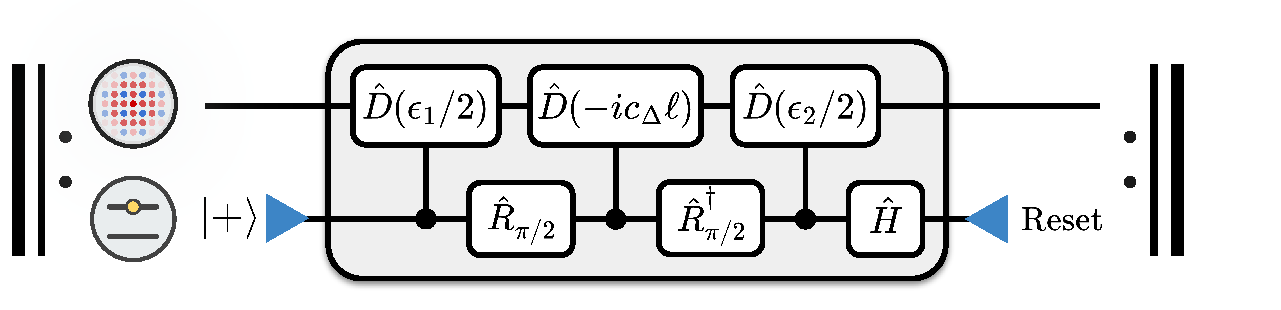
\includegraphics[width=0.85\linewidth]{Figures/2/SBS.pdf}
    \caption{Caption. In certain cases, the final Hadamard can be discarded and absorbed into reset.}
    \label{fig:2-SBS}
\end{figure}

\subsection{The Small-Big-Small (SBS) Protocol}
\textbf{Overview.} The SBS circuit consists of three conditional displacement gates interleaved by qubit rotations. The middle CD involves a large phase space displacement of magnitude $c_\Delta \ell \approx \ell$, and it effectively realizes phase estimation to measure the GKP stabilizer. Here we have defined $c_\Delta \equiv \cosh(\Delta^2)$, and note that $c_\Delta \approx 1$ for all practical values ($\Delta \lesssim 0.4$) of the GKP size. Meanwhile, the first and last CD operations are smaller corrections that account for the finite-energy envelope and perform autonomous error correction respectively (see e.g. \href{https://youtu.be/TOQzHkgsH_E?t=1045}{this talk}). From theory, we have $\epsilon_1 = s_\Delta \ell$ with $s_\Delta \equiv \sinh(\Delta^2) \approx \Delta^2$, and we nominally expect $\epsilon_2 = \epsilon_1$. However, in Ref. \cite{sivak2023gkp-expt}, the authors optimized the two small displacements independently and found, through use of a reinforcement learning (RL) agent, that choosing $\epsilon_2 \gtrsim \epsilon_1$ gave the best QEC performance. This observation has since been corroborated in simulation when accounting for all error channels acting during the SBS unitary, and was also reported in another experiment \cite{nordquantique2023gkp-expt}. Essentially, although $\epsilon_1 = \epsilon_2$ holds for a lossless circuit, when including loss the optimal ratio $\epsilon_2/\epsilon_1$ turns out to be strongly dependent on the actual error channels involved, and is thus another free parameter (like $\Delta$) that can be tweaked in experiment to get the best QEC gain. Finally, it is important to note that the circuit above carries out phase estimation for the $\hat{S}_\Delta^{Z}$ stabilizer; to get the circuit for the $\hat{S}_\Delta^{X}$ stabilizer, we just map ${\rm CD}(\beta) \to {\rm CD}(i\beta)$. The full QEC sequence for SBS then involves repeatedly alternating between the two circuits to stabilize both quadratures. 

\noindent \textbf{Kraus Operators for SBS.} We can describe the SBS protocol in a more quantitative manner by considering it as a quantum channel. To this end, let us imagine that the SBS reset step is implemented using measurement-based active reset. In this case, although the oscillator QEC is still `autonomous', we would have access to the error syndromes by looking at the measurement statistics of the qubit. A subtle yet interesting feature of the circuit above is that---in the absence of errors---it leaves the qubit and oscillator completely disentangled after the unitary evolution (gray box in Fig. \ref{fig:2-SBS}). Thus, if no error occurs, the qubit state will end up in $\ket{g}$ before reset. In our current measurement-based reset approach, then, a measurement outcome $\ket{g}$ would signify ``no error'' while a measurement outcome $\ket{e}$ would imply that an error was detected and corrected. Based on these two outcomes, we can write down the action of the SBS circuit above on just the oscillator by evolving a full qubit-oscillator state through the circuit and then finally tracing out the qubit. This leaves us with a pair of Kraus operators $\hat{K}_g^Z, \hat{K}_e^Z$ for the oscillator, which are given by\footnote{I owe a huge thanks to Jonathan Pelletier for his help deriving these expressions for the general case $\epsilon_1 \neq \epsilon_2$.}:     
\begin{align}
    \begin{split}
        \hat{K}_g^Z &= \cos\bigg(\frac{\epsilon_2 \sqrt{\pi}}{2\sqrt{2}}\bigg)\Bigg[\cos\bigg(\frac{\epsilon_2 + \epsilon_1}{2\sqrt{2}} \hat{p}\bigg)\cos(\sqrt{\pi} \hat{x}) + i\sin\bigg(\frac{\epsilon_2 - \epsilon_1}{2\sqrt{2}} \hat{p}\bigg)\sin(\sqrt{\pi} \hat{x})\Bigg] \\
        &\quad + \sin\bigg(\frac{\epsilon_2 \sqrt{\pi}}{2\sqrt{2}}\bigg)\Bigg[\cos\bigg(\frac{\epsilon_2 - \epsilon_1}{2\sqrt{2}} \hat{p}\bigg)\cos(\sqrt{\pi} \hat{x}) - i\sin\bigg(\frac{\epsilon_2 + \epsilon_1}{2\sqrt{2}} \hat{p}\bigg)\sin(\sqrt{\pi} \hat{x})\Bigg]
    \end{split} \\
    \begin{split}
        \hat{K}_e^Z &= -\cos\bigg(\frac{\epsilon_2 \sqrt{\pi}}{2\sqrt{2}}\bigg)\Bigg[i\sin\bigg(\frac{\epsilon_2 + \epsilon_1}{2\sqrt{2}} \hat{p}\bigg)\cos(\sqrt{\pi} \hat{x}) + \cos\bigg(\frac{\epsilon_2 - \epsilon_1}{2\sqrt{2}} \hat{p}\bigg)\sin(\sqrt{\pi} \hat{x})\Bigg] \\
        &\quad -\sin\bigg(\frac{\epsilon_2 \sqrt{\pi}}{2\sqrt{2}}\bigg)\Bigg[i\sin\bigg(\frac{\epsilon_2 - \epsilon_1}{2\sqrt{2}} \hat{p}\bigg)\cos(\sqrt{\pi} \hat{x}) - \cos\bigg(\frac{\epsilon_2 + \epsilon_1}{2\sqrt{2}} \hat{p}\bigg)\sin(\sqrt{\pi} \hat{x})\Bigg]
    \end{split}
\end{align}
For an input state $\hat{\rho}\otimes \op{+}{+}$ to the SBS circuit, the oscillator state $\hat{\rho}$ after unitary evolution and reset is given by
\begin{equation}
    \hat{\rho} \mapsto \mathcal{R}_\Delta^Z(\hat{\rho}) = \hat{K}_g^Z \hat{\rho} \hat{K}_g^Z{}^\dagger + \hat{K}_e^Z \hat{\rho} \hat{K}_e^Z{}^\dagger  
\end{equation}
where $\mathcal{R}_\Delta^Z$ is the rank-2 dissipator towards the $+1$ eigenspace of $\hat{S}_\Delta^Z$. To get the equivalent dissipator $\mathcal{R}_\Delta^X$ for the stabilizer $\hat{S}_\Delta^X$, we can map $\hat{K}_{g/e}^Z \to \hat{K}_{g/e}^X$ by making the replacement $(x, p) \to (p, -x)$. Finally, the quantum channel for the full SBS QEC cycle is $\mathcal{R}_\Delta = \mathcal{R}_\Delta^X \circ \mathcal{R}_\Delta^Z$. 

In practice, we envision in our experiments using a fully unconditional qubit reset rather than measurement-based feedback. In this case, we won't have access to the measurement statistics (i.e. the protocol will be truly \textit{open-loop}). Furthermore, the final qubit Hadamard gate can be omitted from the protocol and absorbed into the reset operation. Nonetheless, for theoretical analysis and certain numerical simulations, it will make things considerably easier to continue working in the artificial measurement-based feedback picture using the Kraus operators for SBS.

\noindent\textbf{Logical Pauli Measurements.} Just as SBS allowed us to define 

In addition to stabilizer measurements, we can also define qubit-oscillator circuits to perform measurements of the finite-energy logical Pauli operators 

\todo{finish this!}


\section{Implementing Conditional Displacements in Theory}

As we saw in Secs. \ref{sec:2_Intro_to_GKP} and \ref{sec:2_OpenLoopGKPQEC} above, the condition displacement is an essential ingredient for GKP error correction. Therefore, in this section, we will  outline some commonly-used approaches that one can take to realize conditional displacement gates at the Hamiltonian level. The starting point for our discussion is the so-called spin-boson or ``quantum Rabi'' model defined by \cite{hagelstein2004introductory}:
\begin{equation}
\hat{H} = \frac{\omega_q}{2}\sigmaz + \omega_a \hat{a}^\dagger \hat{a} + g\sigmax\big(\hat{a} + \hat{a}^\dagger)
\label{eq:2_QuantumRabiModel_H}
\end{equation}
This Hamiltonian captures the fundamental light-matter interaction between an oscillator and a two-level atom, and it is a model that we will return to and refine when we discuss superconducting qubits and circuit QED in Ch. \ref{ch:3_cQED}. As a brief aside, in the resonant case of $\omega_a \simeq \omega_q$, it is possible to approximate Eq. \eqref{eq:2_QuantumRabiModel_H} by the Jaynes-Cummings model that we saw in Sec. \ref{sec:2_control_nonlinearity_drive}, which has a modified excitation-conserving coupling term $g(\hat{\sigma}_+\hat{a} + \hat{\sigma}_-\hat{a}^\dagger)$; we get to this by expanding $\sigmax = \sigmap + \sigmam$ and performing a rotating-wave approximation to neglect counter-rotating terms [i.e. those that remain fast-oscillating when we move to the rotating frame]. The Rabi model with its dipole coupling $g\sigmax\big(\hat{a} + \hat{a}^\dagger)$ is thus, in a sense, more fundamental than than Jaynes-Cummings model, the latter being an approximation of the former. In what follows, we will try to be careful to highlight whenever the RWA gets invoked.

\subsection{Cross-Resonance Style Conditional Displacement Gates}

Within the general qubit-oscillator model of Eq. \eqref{eq:2_QuantumRabiModel_H}, we can get an effective conditional displacement (CD) interaction $\hat{H}_{\rm CD} = g_{\rm CD}(\hat{a} + \hat{a}^\dagger)\sigmaz$ by coherently driving the qubit at the frequency of the oscillator \cite{touzard2019gated}. We call this a ``cross-resonance'' style CD as the operation principle is identical to that of the cross-resonance gate between two qubits \cite{rigetti2010fully}, in which we start from the static two-qubit Hamiltonian $\hat{H} = \hat{H}_a + \hat{H}_b + g\sigmax^a\sigmax^b$ and drive qubit $b$ at the frequency of qubit $a$ to get an effective interaction of the form  $\hat{H}_{\rm CR} = g_{\rm CR}\sigma_x^a\sigma_z^b$, which we should note is the same as $\hat{H}_{\rm CD}$ if we truncate the oscillator to its lowest levels $\hat{a} + \hat{a}^\dagger \to \sigma_x^a$. In this sense, it does not matter what modes $a$ and $b$ are (i.e. qubits or oscillators) and so the following derivation can be done for any kind of qubit mode $b$, e.g. a fluxonium qubit or a transmon as was considered in Ref. \cite{touzard2019gated}. Here, however, we will present the simplest case of a two-level qubit. We start with the Hamiltonian of Eq. \eqref{eq:2_QuantumRabiModel_H} and add to it a drive term:
\begin{equation}
\hat{H}_0(t) = \frac{\omega_q}{2}\sigmaz + \omega_a \hat{a}^\dagger \hat{a} + g\sigmax\big(\hat{a} + \hat{a}^\dagger) + \Omega \cos(\omega t)\sigmax
\label{eq:CR_CR_initial_eq}
\end{equation}
Here, the phenomenological drive term is of similar nature to the oscillator drives we saw in Sec. \ref{sec:2_control_nonlinearity_drive}. We can transfer the time-dependence of the drive to the coupling by moving to a rotating frame of the qubit at the drive frequency $\omega$. This is done via a unitary operator $\hat{U}_1(t) = \exp[i\omega t \sigmaz / 2] = \cos(\omega t/2)\I +i\sin(\omega t/2)\sigmaz$ to map $\hat{H}_0(t) \mapsto \hat{H}_1 = \hat{U}_1\hat{H}_0\hat{U}_1^\dagger + i[\partial_t \hat{U}_1]\hat{U}_1^\dagger$. We can do this transformation term-by-term  via $\hat{U}_1\sigmax\hat{U}_1^\dagger = \cos(\omega t)\sigmax - \sin(\omega t)\sigmay$ and, since $\sigmaz$ and $\hat{U}_1$ commute, $\hat{U}_1\sigmaz\hat{U}_1^\dagger = \sigmaz$. Defining the detuning $\delta_q = \omega_q - \omega$, the new Hamiltonian is then: 
\begin{equation}
H_1^{\rm RWA} = \frac{\delta_q}{2}\sigmaz + \frac{\Omega}{2}\sigmax + \omega_a \hat{a}^\dagger \hat{a} + g\big[\cos(\omega t)\sigmax - \sin(\omega t)\sigmay\big]\big(\hat{a} + \hat{a}^\dagger)
\end{equation}
Here, we hightlight a rotating-wave approximation (RWA) that was made to simplify\footnote{We can compare to Sec. \ref{sec:2_control_nonlinearity_drive} and consider the replacement $\sigmam \to b$ and $\sigmap\to b^\dagger$. Since $\sigmaz = 1-2\sigmap\sigmam$, we can then think of $\hat{U}_1(t)$ like an oscillator rotating frame transformation $\hat{U}_1(t) = \exp[-i\omega t \sigmap\sigmam]$ which maps $\sigmam \mapsto \sigmam e^{i\omega t}$. This is fully equivalent to the action of $\hat{U}_1$ on the other Paulis above. After the RWA, the simplified drive term reads $(\Omega/2)[\sigmam + \sigmap] = (\Omega/2)\sigmax$. Using intuition from oscillators to reason about qubit frame transformations is an important trick to keep in our toolbox, whenever it is rigorously allowed!} the drive term from $\Omega \cos(\omega t)\sigmax \to (\Omega/2)[\sigmam e^{-i\omega t} + \sigmap e^{i\omega t}]$, i.e. dropping fast oscillating terms at frequencies $\pm 2\omega$. Following \cite{rigetti2010fully}, we can now rotate the quantization axis specified by $(\delta_q\sigmaz + \Omega\sigmaz)/2$ onto the qubit's X-axis via the static rotation $\hat{U}_2 = \exp[-i\xi_q\sigmay/2]$ by an angle $\xi_q = \tan^{-1}(\delta_q/\Omega)$. The qubit then sees an effective field of $\eta_q = (\delta_q^2 + \Omega^2)^{1/2}$ along its new axis of quantization (the X-axis), i.e. $(\delta_q\sigmaz + \Omega\sigmaz)/2 \mapsto \eta_q\sigmax/2$. The rotated Hamiltonian is
\begin{equation}
\hat{H}_2 = \frac{\eta_q}{2}\sigmax + \omega_a \hat{a}^\dagger \hat{a} + g\Big[\cos(\omega t)\big[\cos(\xi_q)\sigmax -\sin(\xi_q)\sigmaz\big]- \sin(\omega t)\sigmay\Big]\big(\hat{a} + \hat{a}^\dagger)
\end{equation}
in this new frame. At this point, we can further move into a jointly rotating frame to get
\begin{align}
\begin{split}
H_3(t) = g\bigg[\cos(\omega t)\Big\{\cos(\xi_q)\sigma_x -\sin(\xi_a)\big[\cos(\eta_q t)\sigma_z + \sin(\eta_q t)\sigma_y\big]\Big\} \\ - \sin(\omega t)\big[\cos(\eta_q t)\sigma_y - \sin(\eta_q t)\sigma_z\big]\bigg]\cdot\Big(a e^{-i\omega_a t} + a^\dagger e^{i\omega_a t}\Big)
\end{split}
\end{align}
where we specifically transform to a rotating frame at frequency $\eta_q$ for the qubit and $\omega_a$ for the oscillator via unitaries $\hat{U}_3^q(t)$ and $\hat{U}_3^a(t)$ (not shown). At \textit{this} point, we can perform the main RWA of this derivation. We set $\omega = \omega_a$ (driving the qubit at the resonator frequency) and rewrite  $\hat{a} e^{-i\omega_a t} + \hat{a}^\dagger e^{i\omega_a t} = (\hat{a}+\hat{a}^\dagger)\cos(\omega_a t) + i(\hat{a}^\dagger - \hat{a})\sin(\omega_a t)$ for ease of averaging, noting that the RWA here amounts to replacing $\cos(\omega t)\cos(\omega t) \to \frac{1}{2}$ and $\cos(\omega t)\sin(\omega t) \to 0$. Doing this gives
\begin{equation}
\hat{H}_{3, \rm\, eff} = \frac{g\cos(\xi_q)}{2} \sigmax\big(\hat{a}+ \hat{a}^\dagger)
\end{equation}
since this is the only static term that survives the averaging. While this is an effective ``XX'' type coupling, we should remember that we are in a non-standard frame of reference for the qubit. We thus revert the transformation $\hat{U}_2$ to realign with the correct quantization axis, giving:
\begin{equation}
\hat{H}_4 =    \frac{g\cos(\xi_q)}{2} \Big[\cos(\xi_q)\sigmax +\sin(\xi_q)\sigmaz\Big]\big(\hat{a}+\hat{a}^\dagger\big)
\end{equation}
Finally, since the drive is set to $\omega = \omega_a$, we get $\delta_q \triangleq \omega_q - \omega_a = \Delta$, i.e. the detuning between the qubit and the resonator, which in most experimental settings we expect to be large. In this case, $\cos^2(\xi_q)= \Omega^2 / [\Omega^2 + \Delta^2] \approx (\Omega/\Delta)^2$, which quickly goes to zero in the limit of $\Delta$ being large, i.e. $\Omega \ll |\Delta|$. Meanwhile, $\cos(\xi_a)\sin(\xi_a)= \Omega_a\Delta / [\Omega_a^2 + \Delta^2] \approx \Omega_a /\Delta$. Therefore, we are left with
\begin{equation}
\hat{H}_{\rm CD} \approx \frac{g\Omega }{2\Delta} \big(\hat{a}+\hat{a}^\dagger\big)\sigmaz
\end{equation}
We have thus arrived at the desired conditional displacement interaction that we wished to demonstrate, with a CD rate of $g_{\rm CD} = g\Omega/2\Delta$. Note, if we added a phase $\phi$ to the initial qubit drive in Eq. \eqref{eq:CR_CR_initial_eq}, i.e. $\Omega\sigmax\cos(\omega t) \to \Omega\sigmax\cos(\omega t + \phi)$, we would instead have gotten the following:
\begin{equation}
\hat{H}_{\rm CD} \approx \frac{g\Omega }{2\Delta}\bigg[\big(\hat{a}+\hat{a}^\dagger)\cos(\phi) + i(\hat{a}^\dagger -\hat{a})\sin(\phi)\bigg]\sigmaz 
\end{equation}
Therefore, we see that it is possible to generate conditional displacements along both the $X \sim \hat{a}+\hat{a}^\dagger$ and $P \sim i(\hat{a}^\dagger -\hat{a})$ quadratures of the oscillator, just by setting the phase of the drive.

\subsection{Echoed Conditional Displacement (ECD) Gates}

The cross-resonance style CD described above was proposed in the context of circuit QED in Ref. \cite{touzard2019gated} using a transmon control qubit. In practice, though, it invariably also leads to a large \textit{unconditional} displacement of the oscillator in addition to the desired CD interaction, due to (a) additional higher-order Hamiltonian terms that arise and (b) inevitable crosstalk and the effect of physically having a strong drive in the system at the oscillator frequency. This style of CD thus typically also requires a separate ``cancellation drive'' to null out the effective displacement of the oscillator. While not a problem per se, the extra calibration needed here should be kept in mind. 

It turns out, however, that there is a better (in some sense) alternative for realizing CDs that has since been developed in the literature \cite{campagne2020gkp-expt, eickbusch2022fast}. The approach in question is called the echoed conditional displacement (ECD), and it makes use of the dispersive interaction between a qubit and an oscillator that we saw in Sec. \ref{sec:2_control_nonlinearity_drive}. The starting point for ECD is the dispersive Hamiltonian with an additional cavity and qubit drive for universal control. In the rotating frames of both the qubit and oscillator, and making the usual RWA on the drive terms\footnote{Implicit in this definition of the Hamiltonian is the fact that both drives are taken to be resonant here.}, we have 
\begin{equation}
    \hat{H} = \frac{\chi}{2}\hat{a}^\dagger\hat{a}\sigmaz + \epsilon(t)\hat{a}^\dagger + \epsilon^\ast(t)\hat{a} + \hat{\Omega}_q(t)
\end{equation}
where $\hat{\Omega}_q(t) = \Omega(t)\sigmap + \Omega^\ast(t)\sigmam$ captures the effect of a general qubit drive. The basic idea behind the ECD approach is to use oscillator displacements as a lever arm in phase space. On its own, the dispersive term $(\chi\sigmaz/2)\hat{a}^\dagger\hat{a}$ generates a conditional \textit{rotation} of the oscillator at frequency $\pm \chi/2$, and we can transform this to a conditional \textit{displacement} as follows via a large phase space displacement. Following \cite{eickbusch2022fast}, we transform $\hat{H}$ above into a displaced frame $\hat{a} \mapsto \hat{a} + \alpha(t)$ where $\alpha(t)$ is determined via the response of the oscillator to the drive\footnote{Specifically, $\alpha(t)$ is determined by the solution to the differential equation $\partial_t\alpha(t) = -i\epsilon(t) - (\kappa/2)\alpha(t)$, with $\kappa$ being the single-photon loss rate. This is the so-called \textit{classical response} of the oscillator to a resonant drive.}. This gives
\begin{equation}
    \hat{H} = \frac{\chi}{2}\hat{a}^\dagger\hat{a}\sigmaz + \frac{\chi}{2}\Big[\alpha(t)\hat{a}^\dagger + \alpha^\ast(t)\hat{a}\Big]\sigmaz + \frac{\chi}{2}|\alpha(t)|^2\sigmaz +  \hat{\Omega}_q(t)
    \label{eq:ECD_disp_frame_H}
\end{equation}
Here, the third term is a Stark-shift of the qubit (i.e. an $\alpha$-dependent frequency shift) while the first and second terms give the new qubit-oscillator interaction in this displaced frame \cite{murch2012cavity, eddins2018stroboscopic}. If $\alpha_{\rm max} = \max|\alpha(t)|$ is large enough, then the second term will dominate over the first and result in the effective qubit-oscillator coupling having the form of a conditional displacement: 
\begin{equation}
    \hat{H} \approx \Big[g_{\rm CD}(t)\hat{a}^\dagger + g_{\rm CD}^\ast(t)\hat{a}\Big]\sigmaz
\end{equation}
with $g_{\rm CD}(t) = \chi\alpha(t)/2$ and a maximum CD rate given by $\chi\alpha_{\rm max}/2$. Of course, we can't just ignore the other terms and so must somehow find a way to cancel them out. The strategy adopted in ECD is to use an ``echo'' sequence which, as depicted in Fig. \ref{fig:2_ECD_pulse_sequence}, consists of a qubit $\pi$-pulse halfway through the evolution [$\ev\sigmaz \to -\ev\sigmaz$] and a flip on the displacement sign $\alpha(t) \to -\alpha(t)$. Intuitively, this can be understood to cancel out all terms in Eq. \eqref{eq:ECD_disp_frame_H} besides the second, which is proportional to $\alpha\sigmaz$ and thus unaffected by the echo, leaving just the desired CD term. More rigorously, there is an exact trajectory in phase space that needs to be implemented via $\epsilon(t)$ and $\Omega(t)$ in order to cancel the unwanted terms, and it can be calculated by solving the Schr\"odinger equation for a given target operation \cite{eickbusch2022fast}. In practice, for finite bandwidth pulses, this typically requires some numerical optimization to compute the correct pulse schedules. In the end, the ECD gate implements the following unitary:
\begin{equation}
    {\rm ECD}(\beta) = \hat{D}\bigg(\frac{\beta}{2}\bigg)\op{e}{g} + \hat{D}\bigg(\frac{-\beta}{2}\bigg)\op{g}{e}
\end{equation}
The time taken to realize a conditional displacement of $\beta$ is approximately $\beta / (\chi\alpha_{\rm max})$, and so it is important to use as large of an intermediate photon number $\alpha_{\rm max}$ as possible to get fast CDs. However, in experiments, there are almost always additional loss channels or unwanted Hamiltonian terms that get activated at large photon numbers, and in practice there is a limit on how large $\alpha_{\rm max}$ can be made before things break. Determining this limit is highly nontrivial; previous GKP experiments have gotten around this by working in the low $\chi$ regime (kHz level) in order to minimize the strength of unwanted nonlinear terms, such as the oscillator's inherited Kerr nonlinearity \cite{campagne2020gkp-expt, eickbusch2022fast, sivak2023gkp-expt, nordquantique2023gkp-expt}. 

\begin{figure}
    \centering
    % \includegraphics{}
    \caption{\todo{make ECD figure}}
    \label{fig:2_ECD_pulse_sequence}
\end{figure}





\todo{Go from JC Hamiltonian to dispersive Hamiltonian, then derive ECD}. Also mention CNOD gates.
In most of what follows, however, we will mainly just consider the far-detuned, or dispersive, limit of Eq. \eqref{eq:2_QuantumRabiModel_H} in which $g \ll |\omega_q - \omega_a|$ and we keep the full Rabi 

\section{Experimental Considerations}

\subsection{Simulations with SBS: I. Oscillator Error Channels}

\subsection{Simulations with SBS: II. Control Qubit Error Channels}

\subsection{Simulations with SBS: III. Kerr and Dispersive Shift}

